\documentclass{beamer}
\usepackage{amsfonts,amsmath,oldgerm}
\usepackage{algpseudocode}
\usepackage{algorithm}
\usepackage{amssymb}
\usepackage{animate}
\usetheme{sintef}

\newcommand{\testcolor}[1]{\colorbox{#1}{\textcolor{#1}{test}}~\texttt{#1}}

\usefonttheme[onlymath]{serif}

\titlebackground*{assets/background}

\newcommand{\hrefcol}[2]{\textcolor{cyan}{\href{#1}{#2}}}

\title{Hindsight Goal Prioritization for Sparse Reward Environments}
\subtitle{Final Project}
\course{Reinforcement Learning}
\author{\href{mailto:maiorana.2051396@studenti.uniroma1.it}{Flavio Maiorana}}
\IDnumber{2051396}
\date{08/09/2023}

\begin{document}
\maketitle

\section{Introduction}

      \begin{frame}{Problem statement}
            \begin{block}{Robotics environments}
                  \begin{itemize}
                        \item Complex and different goals
                        \item Sparse rewards
                        \item Continuous action space
                  \end{itemize}  
            \end{block}

            $\Downarrow$ \centering \\

            \begin{block}{Problems with exploration and reward shaping}
                  \begin{itemize}
                        \item Goal may be too complex and observation space is big: we may never get reward 1
                        \item Classical off-policy algorithms don't valorize much the failed episodes
                  \end{itemize}  
            \end{block}

            $\Downarrow$ \centering \\

            Solution: Enhancing the Replay Buffer
      \end{frame}

      \begin{frame}{Fetch}
            \begin{itemize}
                  \item Based on the 7-DoF Fetch Manipulator arm, with a two-fingered parallel gripper
                  \item Tasks: Reach, Push, Slide and Pick-and-Place
                  \item Action: Box(-1.0, 1.0, (4,), float32) $\rightsquigarrow$ Displacement in meters of the EE 
                  \item Observation: dictionary with info about the robot’s end effector state and goal
                        \begin{itemize}
                              \item Observation: ndarray of shape (25,) $\rightsquigarrow$ kinematic info of the block object and EE
                              \item Desired goal: ndarray of shape (3,) $\rightsquigarrow$ desired position of the EE or the block
                              \item Achieved goal: ndarray of shape (3,) $\rightsquigarrow$ current position of the EE or the block
                        \end{itemize}
                  \item Reward: if we use sparse rewards -1 for every timestep and 0 for reaching the goal
                  \item Termination: episodes have no termination since they have infinite horizon. Thus, they are truncated after T steps (by default 50)
            \end{itemize}
      \end{frame}

\section{DDPG}

      \begin{frame}[fragile]{Architecture - 1}
            \begin{itemize}
                  \item Two neural networks in performing actor-critic policy gradient
                        \begin{itemize}
                              \item \textbf{Actor} $\mu_{\theta}(s_i)$: observed state $\rightarrow$ action maximising the action-value function
                              \item \textbf{Critic} $Q_{\phi}(s_i,\mu_{\theta}(s_i))$: state and action $\rightarrow$ value of the action-value function
                        \end{itemize}
                  \item Experience is collected according to the behavior policy $\pi_b = \mu_{\theta}(s_i) + \mathcal{N}$
                  \item Transitions are stored in a \textbf{replay buffer}
                  \item Every learning step, a batch $B = \{(s_i,a_i,d_i,r_i,s'_i)\}$ is sampled 
            \end{itemize}
      \end{frame}

      \begin{frame}[fragile]{Architecture - 2}
            \begin{itemize}
                  \item Critic optimization through Bellman equation by minimizing
                        \begin{equation}
                              L(\phi) \approx \frac{1}{|B|} \sum_{i=1}^{|B|} \underbrace{\left[ r_i + \gamma Q_{\phi^-}(s'_i,\mu_{\theta^-}(s'_i)) - Q_{\phi}(s_i,a_i)\right]^2}_{\text{Temporal Difference Error}}
                        \end{equation}
                  \item Actor optimization through policy gradient theorem by maximising
                        \begin{equation}
                              J(\theta) \approx \frac{1}{|B|} \sum_{i=1}^{|B|} Q_{\phi}(s_i,\mu_{\theta}(s_i))
                        \end{equation}
                  \item \textbf{Target networks} $\mu_{\theta^-}$ and $Q_{\phi^-}$ for stability, updated with polyak averaging
                        \begin{itemize}
                              \item $Q_{\phi^-} \gets \rho Q_{\phi^-}+ (1-\rho)Q_{\phi}$
                              \item $\mu_{\theta^-} \gets \rho\mu_{\theta^-} + (1-\rho)\mu_{\theta}$
                        \end{itemize}
            \end{itemize}
      \end{frame}


\section{Replay buffer}

      \begin{frame}{Structure}
            \begin{itemize}
                  \item Matrix with $M$ columns and $T$ rows, with $T$ the max number of steps in one episode
                  \item The element $(i,j)$ contains the $j_{th}$ transition of the $i_{th}$ episode
                  \item A transition is defined as $(s_i,a_i,achieved_i,desired_i,r_i,s'_i)$
                  \begin{itemize}
                        \item $achieved_i$ is the current state as if the goal was reached
                        \item $desired_i$ is the actual final goal of the episode
                        \item The reward is computed with $desired_i$
                  \end{itemize}
            \end{itemize}
            \begin{block}{Training steps in Fetch}
                  \begin{itemize}
                        \item For each step in the episode, select an action, clip it to the action space and observe the result of applying it
                        \item Store the episode in a row of the buffer
                        \item Sample |B| transitions, each from a sampled episode
                        \item Do a gradient step
                  \end{itemize}
            \end{block}

            
      \end{frame}

      \begin{frame}[fragile]{HER}
            \begin{itemize}
                  \item The intention is to valorize also failed episodes (majority in robotics environments)
                  \item Done by storing episodes multiple times, substituting the desired goal with a \textbf{Hindsight Goal}, treating the episode as if it was successful
            \end{itemize}
            \begin{block}{Additional steps for HER in DDPG}
                  \begin{itemize}
                        \item Store every transition $\left( s_t||g, a_t, r_t, s_{t+1}||g\right)$ of the episode
                        \item Sample a set of additional achieved goals $G$ from the current episode
                        \item Store $\left( s_t||g', a_t, r_t, s_{t+1}||g'\right)$ for every $g' \in G$
                        \item Perform gradient descent, feeding also the goals into the neural networks
                  \end{itemize}
            \end{block}
            Different strategies can be adopted to sample goals: final, future, random
      \end{frame}

      \begin{frame}[fragile]{HER}
      \framesubtitle{Pseudocode of how transitions are sampled with future strategy}
            \begin{algorithmic}[1]
                  \State $p_{future} \gets 1-\frac{1}{1+k}$ \Comment{k the number of additionally stored episodes: $p_{future} \propto k$} 
                  \State $i_{ep} \gets \text{episodes indices uniformly sampled among the stored ones}$
                  \State $i_{t} \gets \text{transitions indices uniformly sampled from 0 to } T$
                  \State $i_{HER} \gets \text{indices of "resampled" future transitions, according to } p_{future}$
                  \State $i_{future} \gets \text{future transitions indices uniformly sampled from t to } T$
                  \State Substitute $goals[i_{HER}] \text{with a future goal indexed by } i_{future}$
                  \State Recompute the reward of changed transitions
            \end{algorithmic}
      \end{frame}

      \begin{frame}[fragile]{HGR}
            \framesubtitle{Prioritizing future goals}
            \begin{itemize}
                  \item For the $j_{th}$ transition, a transition to be the hindsight goal is sampled according to
                  \begin{equation}
                        P'(j,i) = \frac{|\delta_{ji}|^{\alpha'}}{\sum_{j=0}^{T-2} \sum_{i=j+1}^{T-1}|\delta_{ji}|^{\alpha'}} , \text{ with } j+1 \leq i \leq T-1
                  \end{equation}
                  \item Priorities: matrix of shape $\left(M, \frac{(T-1)\cdot T}{2}\right)$, with $M$ the buffer size in episodes

                  \item New transitions stored with maximal priority, to let them be replayed at least once
            \end{itemize}
      \end{frame}

      \begin{frame}[fragile]{HGR}
            \framesubtitle{Prioritizing episodes}
            \begin{itemize}
                  \item Episodes are sampled according to the probability
                  \begin{equation}
                        P(n) = \frac{|\delta^{(n)}|^{\alpha}}{\sum_{n}|\delta^{(n)}|^{\alpha}}
                  \end{equation} where $|\delta^{(n)}|$ is the average TD Error of an episode
                  \item Sumtree for efficiently sampling from this probability
                  \begin{itemize}
                        \item Priorities in the leaves
                        \item Every node contains the sum of its children
                  \end{itemize}
            \end{itemize}
      \end{frame}

      \begin{frame}{HGR}
            \framesubtitle{Annealing the bias}
            \begin{itemize}
                  \item Importance sampling weights helps to scale down the sample’s gradient when it is updated frequently and remains the same when it is rarely updated
                  \begin{equation}
                        w_{ji}^{(n)} = \left( \frac{1}{N_e}\frac{1}{P(n)}\right) ^{\beta} \cdot \left( \frac{2}{(T-1)\cdot T} \cdot \frac{1}{P'(j,i)}\right) ^ {\beta'}
                  \end{equation}
                  \item In order to always scale the gradients down we set $w_{ji}^{(n)} = \frac{w_{ji}^{(n)}}{max(w_{ji}^{(n)})}$
                  \item Mintree for storing minimum weight, for efficiently retrieving inverse of max weight
            \end{itemize}
            
      \end{frame}


\section{Results}

      \begin{frame}{Training setup}
            \begin{itemize}
                  \item Normal noise with standard deviation 0.2
                  \item $\gamma = 0.98$
                  \item Learning rates 0.001, polyak 0.95
                  \item buffer capacity $1\cdot 10^6$, batch size 256
                  \item gradient steps 50
                  \item $\alpha = \alpha' = 0.6$
                  \item $\beta_0 = \beta' = 0.4$
                  \item $\beta$ organized with linear schedule from $\beta_0$ to 1
            \end{itemize}
      \end{frame}

      \begin{frame}[fragile]{Reach}
            \begin{columns}
                  \column{0.5\textwidth}
                        \centering
                        \animategraphics[width=0.8\columnwidth,loop,controls,autoplay]{10}{videos/reach/reach-}{0}{51}
                  \column{0.5\textwidth}
                  \begin{figure}
                        \centering
                        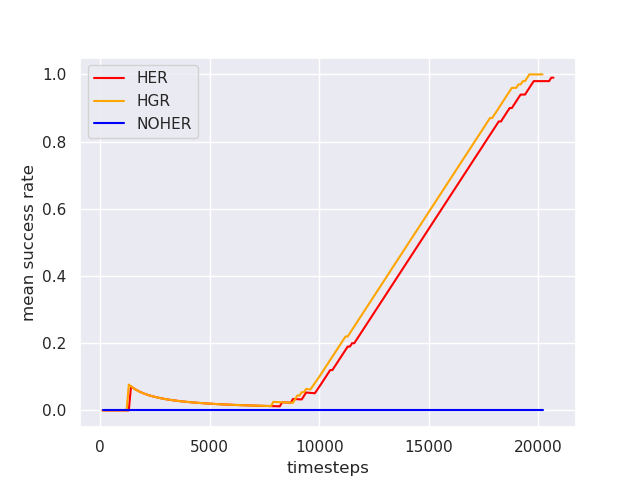
\includegraphics[width=1.1\columnwidth]{figures/reach.png}
                  \end{figure}
            \end{columns}
      \end{frame}

      \begin{frame}{Push}
            \begin{columns}
                  \column{0.5\textwidth}
                        \centering
                        \animategraphics[width=0.8\columnwidth,loop, controls, autoplay]{10}{videos/push/push-}{0}{50}
                  \column{0.5\textwidth}
                  \begin{figure}
                        \centering
                        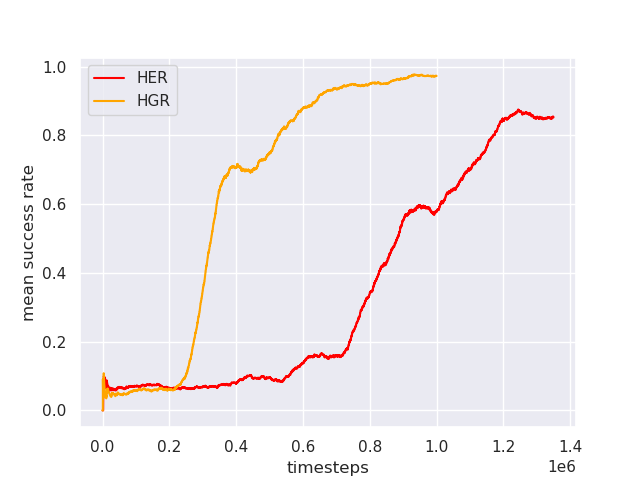
\includegraphics[width=\columnwidth]{figures/push.png}
                  \end{figure}
            \end{columns}
      \end{frame}

      \begin{frame}{Pick-and-Place}
            \begin{columns}
                  \column{0.5\textwidth}
                        \centering
                        \animategraphics[width=0.8\columnwidth,loop,controls, autoplay]{10}{videos/pickandplace/pickandplace-}{0}{50}
                  \column{0.5\textwidth}
                  \begin{figure}
                        \centering
                        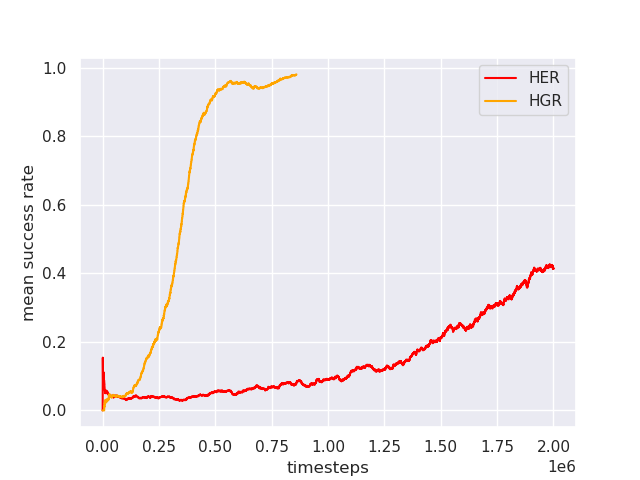
\includegraphics[width=\columnwidth]{figures/pickandplace.png}
                  \end{figure}
            \end{columns}
      \end{frame}

\section{Conclusions}
      \begin{frame}{Final considerations}
            \begin{itemize}
                  \item Sampling additional goals solves the exploration problem in multi-goal sparse reward environments
                  \item Prioritizing episodes and goals makes sampling even more effective and thus significantly reduces training time and the amount of collected experience
            \end{itemize}
      \end{frame}

      \begin{frame}{Resources}
            \begin{itemize}
                  \item T. M. Luu, C. D. Yoo: HGR on Replay Buffer for Sparse Reward Environment
                  \item Marcin Andrychowicz et al. : Hindsight Experience Replay
                  \item Tom Schaul et al. : Prioritized Experience Replay
                  \item \href{https://spinningup.openai.com/en/latest/algorithms/ddpg.html}{OpenAI Spinning Up}
            \end{itemize}
      \end{frame}

\backmatter
\end{document}